%%%%%%%%%%%%%%%%%%%%%%%%%%%%%%%%%%%%%%%%%%%%%%%%%%%%%%%%%%%%
%  HOMEWORK / REPORT PREAMBLE  (two-column, ML-paper style)
%  Derived from Classes_TEX/_system/templates/preamble_notes.tex.
%  Changes vs. the notes preamble: Times text+math (newtx), letter paper,
%  slightly wider margins, paper-style title block, natbib author-year
%  citations, no lecture/figure-card/provenance machinery.
%
%  Math convention: French formatting.
%    \intint{1}{N}  -> [[1,N]]   (integer interval)
%    \oo{a}{b} ]a,b[   \oc{a}{b} ]a,b]   \co{a}{b} [a,b[   \cc{a}{b} [a,b]
%    \leq/\geq are slanted (\leqslant/\geqslant); R_+^* for positive reals.
%%%%%%%%%%%%%%%%%%%%%%%%%%%%%%%%%%%%%%%%%%%%%%%%%%%%%%%%%%%%
\documentclass[10pt,twocolumn]{article}
\usepackage[letterpaper,margin=0.7in,top=0.85in,bottom=0.85in,columnsep=0.25in]{geometry}
\usepackage[T1]{fontenc}
\usepackage[utf8]{inputenc}
\usepackage{amsmath,amssymb,amsthm,mathtools}
\usepackage{newtxtext}
\usepackage[varbb]{newtxmath}
\usepackage{bm}
\usepackage{stmaryrd}        % \llbracket \rrbracket
\usepackage{microtype}
\usepackage{graphicx}
\usepackage{enumitem}
\usepackage{booktabs}
\usepackage{array}
\usepackage{multirow}
\usepackage{tabularx}
\usepackage{tikz}
\usepackage{pgfplots}
\usepackage{mdframed}
\usepackage{xcolor}
\usepackage[sort&compress]{natbib}
\usepackage{hyperref}
\usepackage[nameinlink,noabbrev]{cleveref}
\usepackage{titlesec}
\usepackage{fancyhdr}
\usepackage{lastpage}
\usepackage{caption}
\pgfplotsset{compat=1.18}
\usetikzlibrary{arrows.meta,positioning,calc,patterns}

\definecolor{linkblue}{RGB}{20,60,140}
\definecolor{boxgray}{gray}{0.965}
\definecolor{linegray}{gray}{0.72}
\hypersetup{colorlinks=true,linkcolor=linkblue,citecolor=linkblue,urlcolor=linkblue}

%%%%%%%%%%%%%%%%%%%%%%%%%%%%%%%%%%%%%%%%%%%%%%%%%%%%%%%%%%%%
%  Citations / bibliography (author-year, ML style)
%%%%%%%%%%%%%%%%%%%%%%%%%%%%%%%%%%%%%%%%%%%%%%%%%%%%%%%%%%%%
\setcitestyle{authoryear,round,citesep={;},aysep={,},yysep={,}}
\bibliographystyle{plainnat}
\renewcommand{\bibfont}{\footnotesize}
\setlength{\bibsep}{1.5pt plus 0.5pt}

%%%%%%%%%%%%%%%%%%%%%%%%%%%%%%%%%%%%%%%%%%%%%%%%%%%%%%%%%%%%
%  Theorem-like environments
%%%%%%%%%%%%%%%%%%%%%%%%%%%%%%%%%%%%%%%%%%%%%%%%%%%%%%%%%%%%
\theoremstyle{plain}
\newtheorem{theorem}{Theorem}
\newtheorem{proposition}[theorem]{Proposition}
\newtheorem{lemma}[theorem]{Lemma}
\newtheorem{corollary}[theorem]{Corollary}
\newtheorem{claim}[theorem]{Claim}
\theoremstyle{definition}
\newtheorem{definition}[theorem]{Definition}
\newtheorem{assumption}[theorem]{Assumption}
\theoremstyle{remark}
\newtheorem{remark}[theorem]{Remark}

%%%%%%%%%%%%%%%%%%%%%%%%%%%%%%%%%%%%%%%%%%%%%%%%%%%%%%%%%%%%
%  Section formatting (ICML-like: numbered, bold, compact)
%%%%%%%%%%%%%%%%%%%%%%%%%%%%%%%%%%%%%%%%%%%%%%%%%%%%%%%%%%%%
\titleformat{\section}{\large\bfseries}{\thesection}{0.6em}{}
\titleformat{\subsection}{\normalsize\bfseries}{\thesubsection}{0.5em}{}
\titleformat{\subsubsection}{\normalsize\bfseries\itshape}{\thesubsubsection}{0.5em}{}
\titleformat{\paragraph}[runin]{\normalsize\bfseries}{}{0pt}{}[.]
\titlespacing*{\section}{0pt}{8pt plus 2pt minus 1pt}{4pt}
\titlespacing*{\subsection}{0pt}{6pt plus 1pt minus 1pt}{3pt}
\titlespacing*{\subsubsection}{0pt}{5pt plus 1pt minus 1pt}{2pt}
\titlespacing*{\paragraph}{0pt}{4pt plus 1pt minus 1pt}{0.6em}

%%%%%%%%%%%%%%%%%%%%%%%%%%%%%%%%%%%%%%%%%%%%%%%%%%%%%%%%%%%%
%  Layout (paper-style: indented paragraphs, compact lists)
%%%%%%%%%%%%%%%%%%%%%%%%%%%%%%%%%%%%%%%%%%%%%%%%%%%%%%%%%%%%
\setlength{\parindent}{1em}
\setlength{\parskip}{1pt plus 0.5pt}
\AtBeginDocument{%
  \setlength{\abovedisplayskip}{4pt plus 1pt minus 1pt}%
  \setlength{\belowdisplayskip}{4pt plus 1pt minus 1pt}%
  \setlength{\abovedisplayshortskip}{2pt plus 1pt}%
  \setlength{\belowdisplayshortskip}{2pt plus 1pt}}
\setlength{\textfloatsep}{8pt plus 2pt minus 2pt}
\setlength{\floatsep}{6pt plus 2pt minus 2pt}
\setlength{\intextsep}{6pt plus 2pt minus 2pt}
\setlist[itemize]{topsep=2pt,itemsep=1pt,parsep=0pt,leftmargin=1.2em}
\setlist[enumerate]{topsep=2pt,itemsep=1pt,parsep=0pt,leftmargin=1.4em}
\setlist[description]{topsep=2pt,itemsep=1pt,parsep=0pt,leftmargin=1em}
\captionsetup{font=small,labelfont=bf,skip=3pt}
\raggedbottom

%%%%%%%%%%%%%%%%%%%%%%%%%%%%%%%%%%%%%%%%%%%%%%%%%%%%%%%%%%%%
%  Boxes
%%%%%%%%%%%%%%%%%%%%%%%%%%%%%%%%%%%%%%%%%%%%%%%%%%%%%%%%%%%%
\newmdenv[
  backgroundcolor=boxgray,linecolor=linegray,linewidth=0.5pt,
  topline=false,bottomline=false,rightline=false,leftline=true,linewidth=1.2pt,
  innertopmargin=4pt,innerbottommargin=4pt,innerleftmargin=6pt,innerrightmargin=6pt,
  skipabove=5pt,skipbelow=5pt
]{keybox}
\newenvironment{question}[1][Question]{\begin{keybox}\textbf{#1.} }{\end{keybox}}

%%%%%%%%%%%%%%%%%%%%%%%%%%%%%%%%%%%%%%%%%%%%%%%%%%%%%%%%%%%%
%  Math macros (French conventions)
%%%%%%%%%%%%%%%%%%%%%%%%%%%%%%%%%%%%%%%%%%%%%%%%%%%%%%%%%%%%
\let\leq\leqslant \let\le\leqslant
\let\geq\geqslant \let\ge\geqslant
\newcommand{\intint}[2]{\llbracket #1, #2 \rrbracket}
\newcommand{\oo}[2]{\left]#1, #2\right[}
\newcommand{\oc}[2]{\left]#1, #2\right]}
\newcommand{\co}[2]{\left[#1, #2\right[}
\newcommand{\cc}[2]{\left[#1, #2\right]}
\newcommand{\R}{\mathbb{R}}
\newcommand{\N}{\mathbb{N}}
\newcommand{\Z}{\mathbb{Z}}
\newcommand{\E}{\mathbb{E}}
\newcommand{\Prob}{\mathbb{P}}
\newcommand{\eps}{\varepsilon}
\newcommand{\ind}{\mathbf{1}}
\newcommand{\T}{\top}
\DeclarePairedDelimiter{\abs}{\lvert}{\rvert}
\DeclarePairedDelimiter{\norm}{\lVert}{\rVert}
\DeclarePairedDelimiter{\ip}{\langle}{\rangle}
\DeclarePairedDelimiter{\set}{\lbrace}{\rbrace}
\DeclareMathOperator{\Var}{Var}
\DeclareMathOperator{\Cov}{Cov}
\DeclareMathOperator{\tr}{tr}
\DeclareMathOperator{\diag}{diag}
\DeclareMathOperator*{\argmin}{arg\,min}
\DeclareMathOperator*{\argmax}{arg\,max}
\newcommand{\grad}{\nabla}

%%%%%%%%%%%%%%%%%%%%%%%%%%%%%%%%%%%%%%%%%%%%%%%%%%%%%%%%%%%%
%  Title block and running heads
%  \settitle{Title}{Running head}  \setauthors{...}  \setcourse{...}
%  \setdate{...}  then \makeheader[optional abstract text]
%%%%%%%%%%%%%%%%%%%%%%%%%%%%%%%%%%%%%%%%%%%%%%%%%%%%%%%%%%%%
\makeatletter
\newcommand{\@doctitle}{}\newcommand{\@runhead}{}
\newcommand{\settitle}[2]{\renewcommand{\@doctitle}{#1}\renewcommand{\@runhead}{#2}}
\newcommand{\@docauthors}{}\newcommand{\setauthors}[1]{\renewcommand{\@docauthors}{#1}}
\newcommand{\@doccourse}{}\newcommand{\setcourse}[1]{\renewcommand{\@doccourse}{#1}}
\newcommand{\@docdate}{\today}\newcommand{\setdate}[1]{\renewcommand{\@docdate}{#1}}
\newcommand{\makeheader}[1][]{%
  \twocolumn[{%
    \begin{center}
      \vspace*{-0.35in}
      {\LARGE\bfseries \@doctitle\par}\vspace{7pt}
      {\normalsize \@docauthors\par}\vspace{2pt}
      {\small\itshape \@doccourse\ \textperiodcentered\ \@docdate\par}
    \end{center}
    \if\relax\detokenize{#1}\relax\else
      \begin{center}\begin{minipage}{0.86\textwidth}\small
        \textbf{Abstract.} #1
      \end{minipage}\end{center}
    \fi
    \vspace{2pt}\noindent\rule{\textwidth}{0.4pt}\vspace{8pt}
  }]%
  \thispagestyle{plain}%
}
\pagestyle{fancy}
\fancyhf{}
\fancyhead[L]{\small\itshape \@doccourse}
\fancyhead[R]{\small\itshape \@runhead}
\fancyfoot[C]{\small \thepage/\pageref*{LastPage}}
\renewcommand{\headrulewidth}{0.3pt}
\renewcommand{\footrulewidth}{0pt}
\fancypagestyle{plain}{\fancyhf{}\fancyfoot[C]{\small \thepage/\pageref*{LastPage}}%
  \renewcommand{\headrulewidth}{0pt}}
\makeatother

%%%%%%%%%%%%%%%%%%%%%%%%%%%%%%%%%%%%%%%%%%%%%%%%%%%%%%%%%%%%
%  Project-specific additions (FinEng P1)
%%%%%%%%%%%%%%%%%%%%%%%%%%%%%%%%%%%%%%%%%%%%%%%%%%%%%%%%%%%%
\graphicspath{{../figures/}}
\usepackage{needspace}
\usepackage{placeins}
\newenvironment{takeaway}{\begin{keybox}\textbf{Key result.} }{\end{keybox}}
\newcommand{\bp}{\,bp}

\renewcommand{\topfraction}{0.9}\renewcommand{\dbltopfraction}{0.9}\renewcommand{\textfraction}{0.08}
\renewcommand{\floatpagefraction}{0.8}\renewcommand{\dblfloatpagefraction}{0.8}
\setcounter{dbltopnumber}{3}


\settitle{On a Model for Normal and Inverted Yield Curves}{Project 1: Yield Curve}
\setauthors{Arturo Favara, Nick Bernardini, Clarys Vignal}
\setcourse{15.456 Financial Engineering, Fall 2026 \quad Independent Project 1, Topic 4}
\setdate{13 November 2026}

\begin{document}

% Sharing consent (uncomment if you agree):
% \noindent\textit{We, Arturo Favara, Nick Bernardini and Clarys Vignal, consent to future use of our report for educational purposes within the scope of the MFin program. The report may be shared with MFin students, teaching assistants, and faculty.}

\makeheader

%==============================================================================
\section*{Executive summary}
\begin{keybox}
Long-term borrowing usually costs more than short-term borrowing. From late 2022 to 2025 it didn't: for 30 months, the longest stretch on record, three-month Treasury bills yielded more than ten-year notes. Every such ``inversion'' since 1969 had been followed by a recession. This one wasn't. We asked whether one pricing model, with one set of parameters, can describe both normal and inverted curves.

\begin{itemize}
  \item \textbf{The simplest model (one random interest rate) cannot.} It fits a single day only by using implausible inputs, and with fixed inputs its errors reach 0.5--0.8 percentage points.
  \item \textbf{A model with two drivers can.} One sets the general level of rates, the other the gap between short and long rates. With one set of parameters it fits every month from 1990 to 2026 to about 0.14 points, and it is just as accurate when the curve is inverted.
  \item \textbf{An inversion is the second driver at an extreme.} In 2023 between half and two-thirds of it reflected expected rate cuts, the rest an unusually low premium for holding long bonds. The cuts it priced did come, a year late. Statistical models read it as roughly a coin flip for recession (47--58\%), the strongest warning since the early 1980s; the outcome landed on the other side.
  \item \textbf{The model is useful in practice.} It prices bonds it was not fitted to almost as well as those it was. A hedge based on its two drivers removes 91--96\% of a ten-year bond's daily risk, against 40--89\% for the standard one-number (duration) hedge.
\end{itemize}
\end{keybox}

%==============================================================================
\section{Introduction}

\begin{figure*}[t]
  \centering
  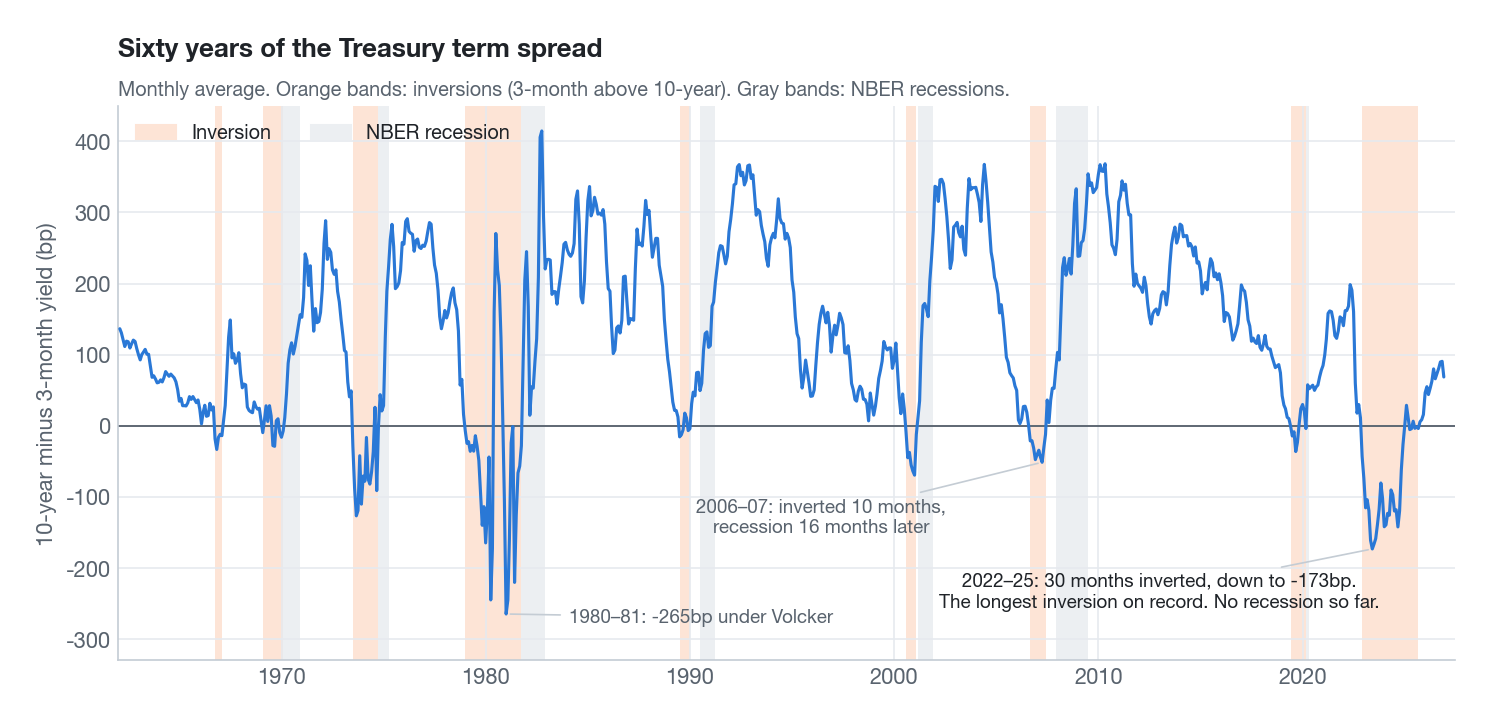
\includegraphics[width=0.82\textwidth]{hero_spread-light.png}
  \caption{The ten-year minus three-month Treasury yield, 1962--2026. Inversions (orange) preceded every recession (gray) since 1969. The 2022--25 inversion was the longest on record and has not been followed by one.}
  \label{fig:hero}
\end{figure*}

An investor who lends for ten years gives up flexibility and bears more interest-rate risk than one who lends for three months, so long yields should normally exceed short ones. Yet from November 2022 to August 2025 the three-month Treasury yield was above the ten-year yield in 30 of 34 months, by up to 1.7 percentage points (\cref{fig:hero}). The usual reading is that an inverted curve prices in rate cuts because a recession is coming. Nine inversions since 1962 support it; the latest one did not.

\paragraph{Question} Can a single no-arbitrage model, with one set of parameters, describe both normal and inverted curves? If so, what does it need?

\paragraph{Expectations} In the one-factor Vasicek model from class, an inversion just means the short rate sits above its long-run mean, so in theory one model covers both regimes. In practice we expected two problems. First, one factor allows at most one hump, but real curves sometimes change direction twice. Second, the volatility that fits a curve's shape need not match how rates actually move.

\paragraph{Approach} We fit a ladder of models, each adding one feature, to the prices of every Treasury on five dates covering every curve shape since 2006, and then to 37 years of monthly curves with a single parameter set. We then separate expected rates from the term premium, use the curves to price and hedge, and as a bonus examine how the curve moves within minutes of Fed and data announcements.

%==============================================================================
\section{Scope}

U.S.\ Treasury nominal bills, notes and bonds (no TIPS, callable or flower bonds). \textbf{Models:} Nelson-Siegel and Svensson as curve-fitting benchmarks (not arbitrage-free); Vasicek, CIR and the two-factor Gaussian G2++ as no-arbitrage models; Dynamic Nelson-Siegel as a three-factor reference. \textbf{Fitting dates:} Dec 2006 (mild inversion), Jun 2021 (steep, zero short rate), Jun 2023 (deep inversion), Sep 2024 (U-shape), Jun 2026 (normal), then every month-end from 1990 (1971 for robustness) to Oct 2026. \textbf{Uses:} pricing bonds, hedging a ten-year note, pricing a bond option, and announcement-day behavior (2018--2026).

%==============================================================================
\section{Data}

\begin{table}[h]
\centering\small
\begin{tabularx}{\columnwidth}{@{}lX@{}}
\toprule
Source & Use \\
\midrule
CRSP Treasury (WRDS) & bid/ask, coupon and maturity of every Treasury, daily 1961--Jun 2026; model fits, hedging \\
Fed zero curve \citep{gsw2007} & daily zero yields 1--30y, 1961--2026; monthly panel, factors \\
Fed H.15 + U.S.\ Treasury & constant-maturity yields 1962--2026; inversions, short end \\
NY Fed ACM & published term premium; validation only \\
NYSE TAQ (WRDS) & millisecond quotes of Treasury ETFs, 562 days; announcements \\
\bottomrule
\end{tabularx}
\end{table}

\begin{figure*}[t]
  \centering
  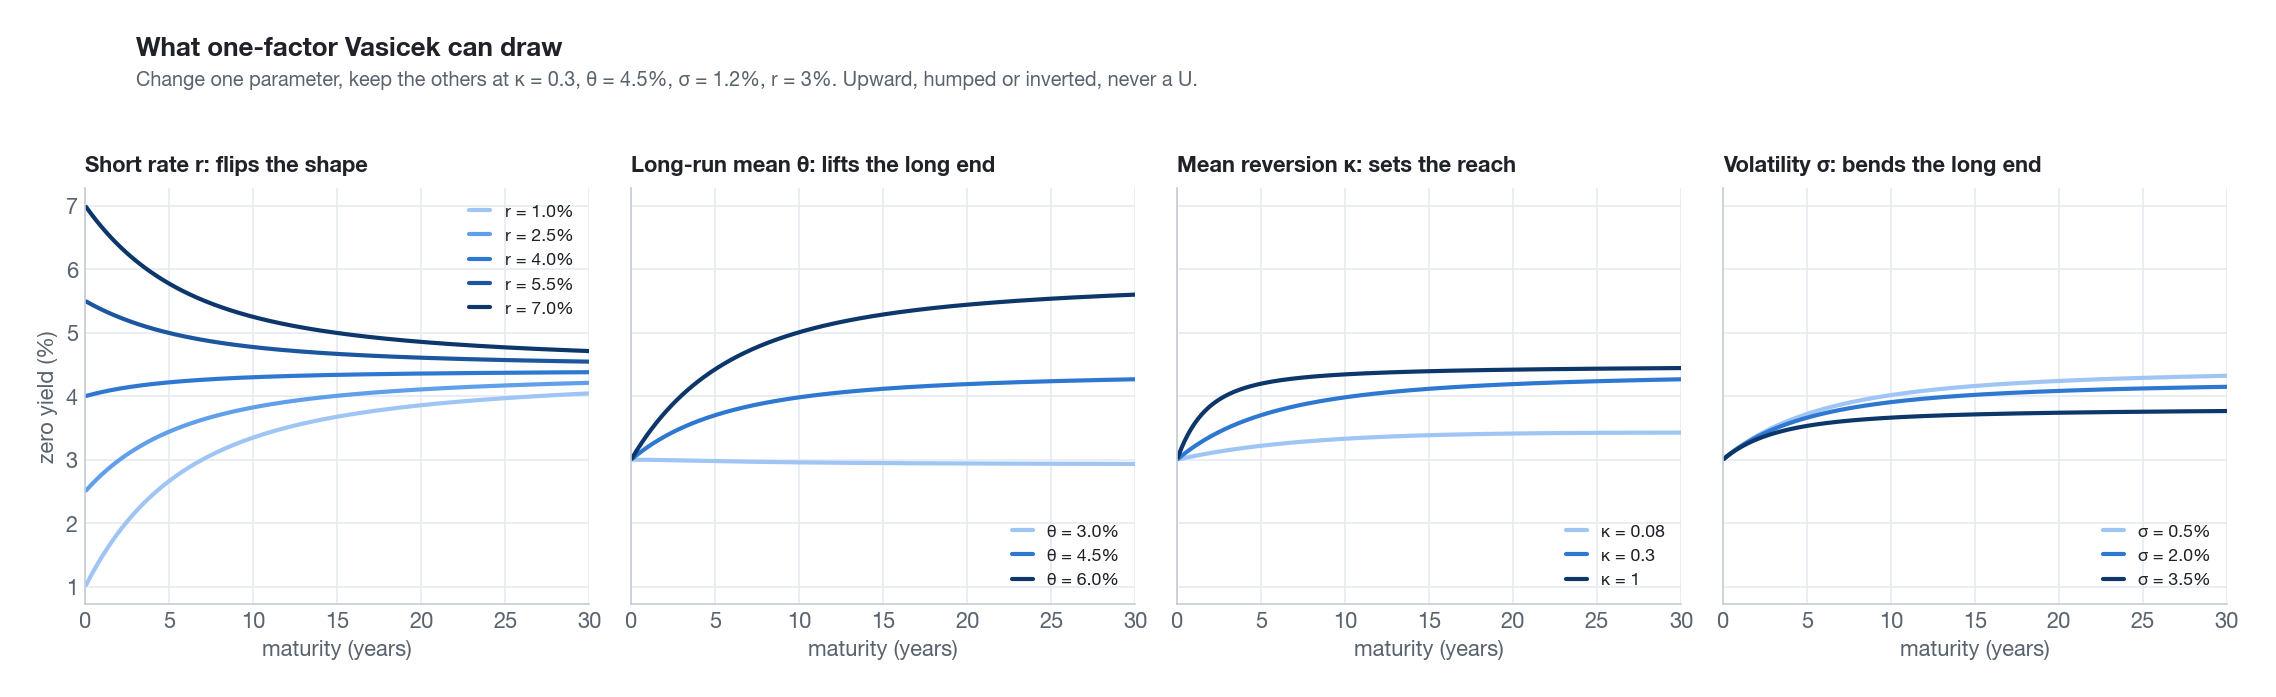
\includegraphics[width=0.82\textwidth]{vasicek_shapes-light.png}
  \caption{What one-factor Vasicek can draw. Each panel changes one parameter (others at $\kappa=0.3$, $\theta=4.5\%$, $\sigma=1.2\%$, $r=3\%$). Only the short rate flips the curve between upward and inverted; no parameter produces a U.}
  \label{fig:shapes}
\end{figure*}

\noindent We chose CRSP because it has individual bond prices, so fits are judged on what actually trades rather than on a pre-smoothed curve. On each date we kept non-callable, fully taxable nominal issues that had already been issued, with at least 30 days to maturity for bills and one year for notes and bonds. Short coupon issues are old and illiquid: one note due in a month showed a 3.5\% yield while bills yielded 5.3\%. This leaves 150--340 securities per date. Prices are the bid/ask midpoint plus accrued interest. For the monthly panel (442 months) we combine the Fed's 1--30 year zero yields with the 3- and 6-month bill yields, converted to continuous compounding. Inversion episodes use the 10-year minus 3-month spread, with gaps of up to seven months merged. The data-extraction scripts and analysis code are available on request, so every number here can be reproduced.

%==============================================================================
\section{Models and methods}

\paragraph{Vasicek} Under the pricing measure $Q$ the short rate follows $dr = \kappa(\theta - r)\,dt + \sigma\,dW$, and the zero-coupon yield for maturity $\tau$ is
\begin{equation}
  y(\tau) = y_\infty + (r - y_\infty)\frac{B(\tau)}{\tau} + \frac{\sigma^2}{4\kappa}\frac{B(\tau)^2}{\tau},
  \label{eq:vas}
\end{equation}
with $B(\tau) = (1-e^{-\kappa\tau})/\kappa$ and $y_\infty = \theta - \sigma^2/2\kappa^2$ \citep{vasicek1977}. The curve is upward if $r < y_\infty - \sigma^2/4\kappa^2$, inverted if $r > y_\infty + \sigma^2/2\kappa^2$, and humped in between. It can never form a U. A change in $r$ moves yields by $B/\tau$ (fading with maturity) and a change in $\theta$ by $1 - B/\tau$ (growing with maturity). \emph{Equal moves in $r$ and $\theta$ shift the curve in parallel; opposite moves tilt it.} $\sigma$ only bends the long end down. CIR (Cox, Ingersoll and Ross) replaces $\sigma$ with $\sigma\sqrt{r}$ and keeps rates positive (\cref{fig:shapes}).

\begin{figure*}[t]
  \centering
  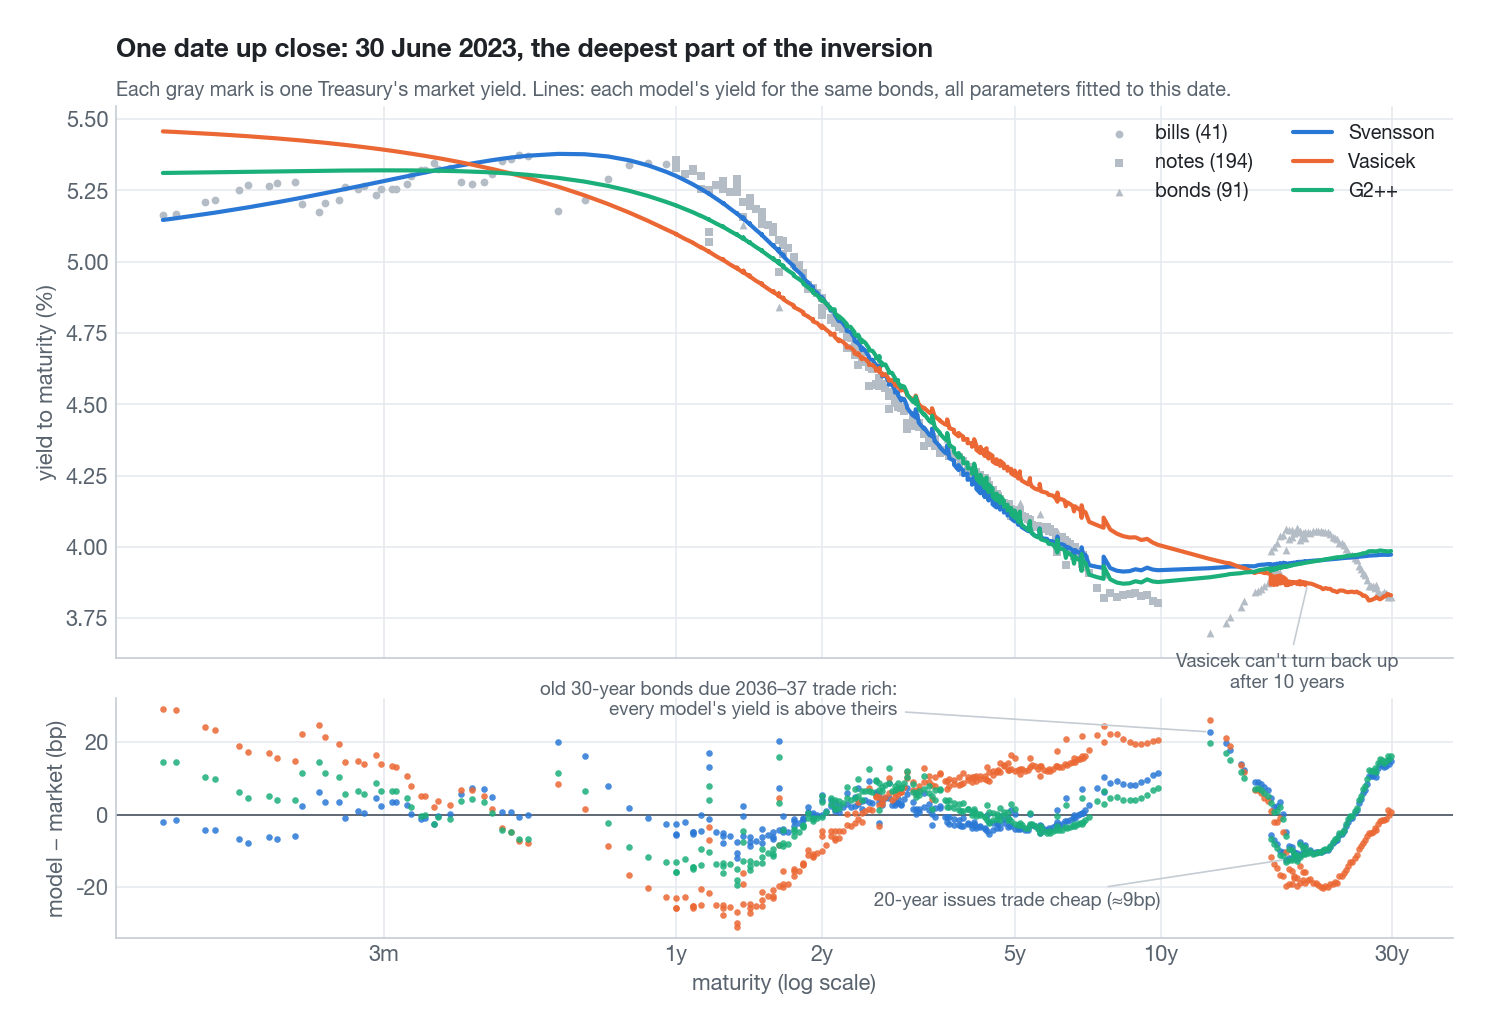
\includegraphics[width=0.64\textwidth]{june2023_closeup-light.png}
  \caption{30 June 2023, the deepest inversion. Gray marks: market yields of 326 Treasuries. Lines: each model's yield for the same bonds. Bottom: errors per bond.}
  \label{fig:jun23}
\end{figure*}

\paragraph{G2++} The short rate is $r = \delta + x_1 + x_2$, where $x_1, x_2$ are mean-reverting Gaussian factors with speeds $a_1, a_2$, volatilities $\sigma_1, \sigma_2$ and correlation $\rho$ \citep{brigo2006}. Zero yields are affine: $y(\tau) = a(\tau) + \tfrac{B_1(\tau)}{\tau} x_1 + \tfrac{B_2(\tau)}{\tau} x_2$. A slow and a fast factor together can draw a U.

\paragraph{Assumptions} All three no-arbitrage models assume frictionless markets with no arbitrage, bond prices computed as expectations under a risk-neutral measure $Q$, parameters constant over time, and a short rate driven by one (Vasicek, CIR) or two (G2++) Brownian factors. Vasicek and G2++ rates are Gaussian and can turn negative; CIR rates cannot.

\begin{figure*}[t]
  \centering
  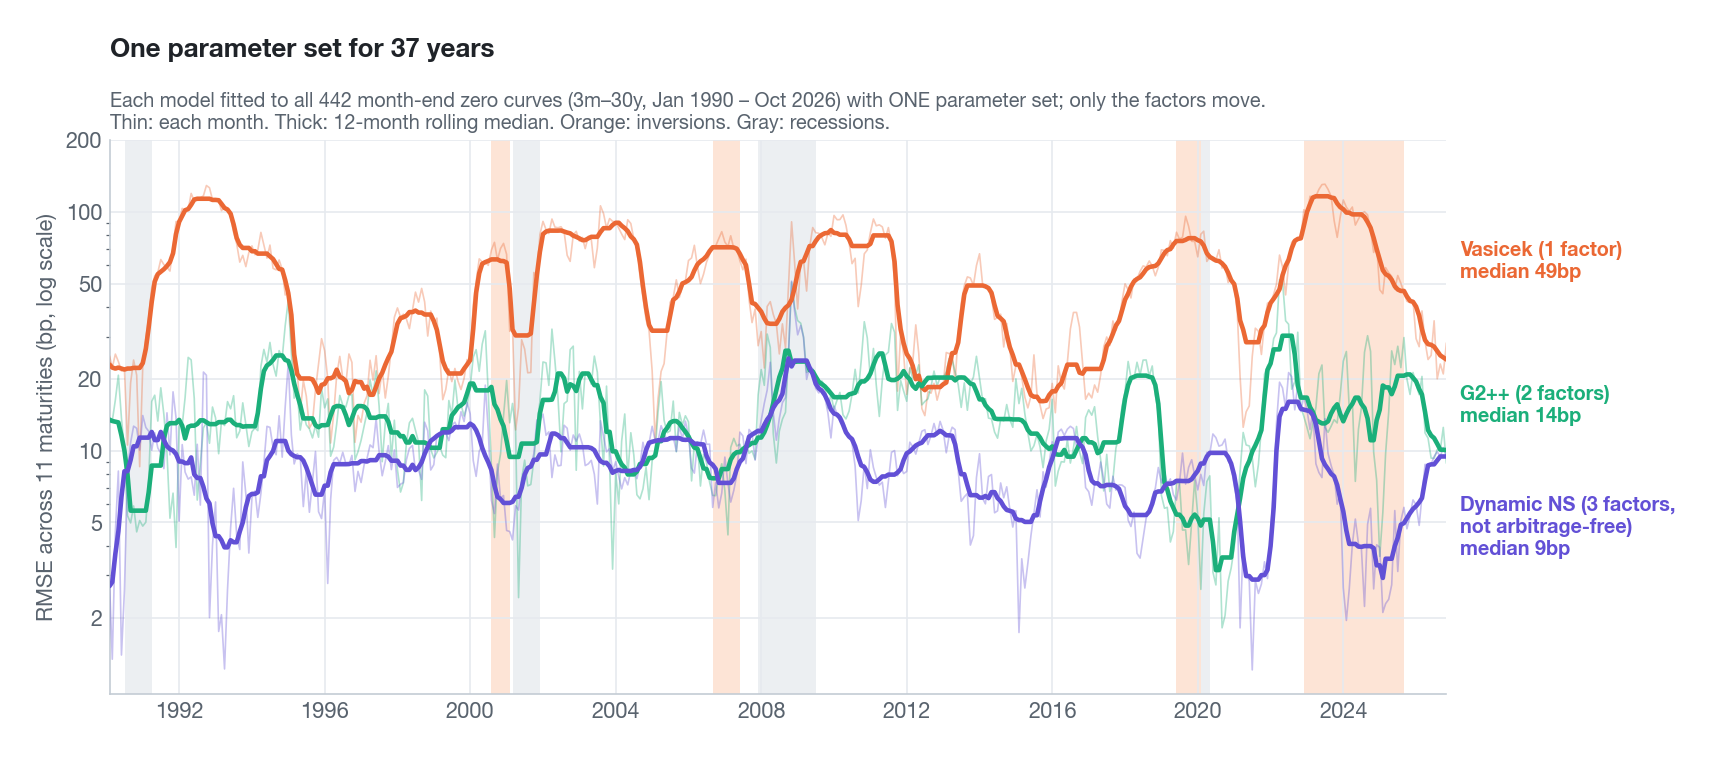
\includegraphics[width=0.70\textwidth]{through_time_rmse-light.png}
  \caption{Monthly fit error, Jan 1990--Oct 2026, with one parameter set per model for all 442 months (thin: each month; thick: 12-month median; orange: inversions).}
  \label{fig:time}
\end{figure*}

\paragraph{Fitting} Each bond is priced by discounting its cash flows on the model curve. We minimize duration-weighted price errors, which to first order are errors in each bond's yield, and report model minus market yield in basis points (bp). All computations are in Python: SciPy nonlinear least squares for the fits, NumPy for the VAR, statsmodels for the probits, and a Monte Carlo simulation to check the option formula. We run two tests. \emph{Per date:} all parameters are refitted on each date. \emph{Shared:} one structural parameter set $(\kappa,\theta,\sigma)$ or $(a_1,a_2,\sigma_1,\sigma_2,\rho,\delta)$ for every date, with only the state ($r$ or $x_1,x_2$) varying. The shared test is the brief's ``one model'' question.

\begin{figure*}[t]
  \centering
  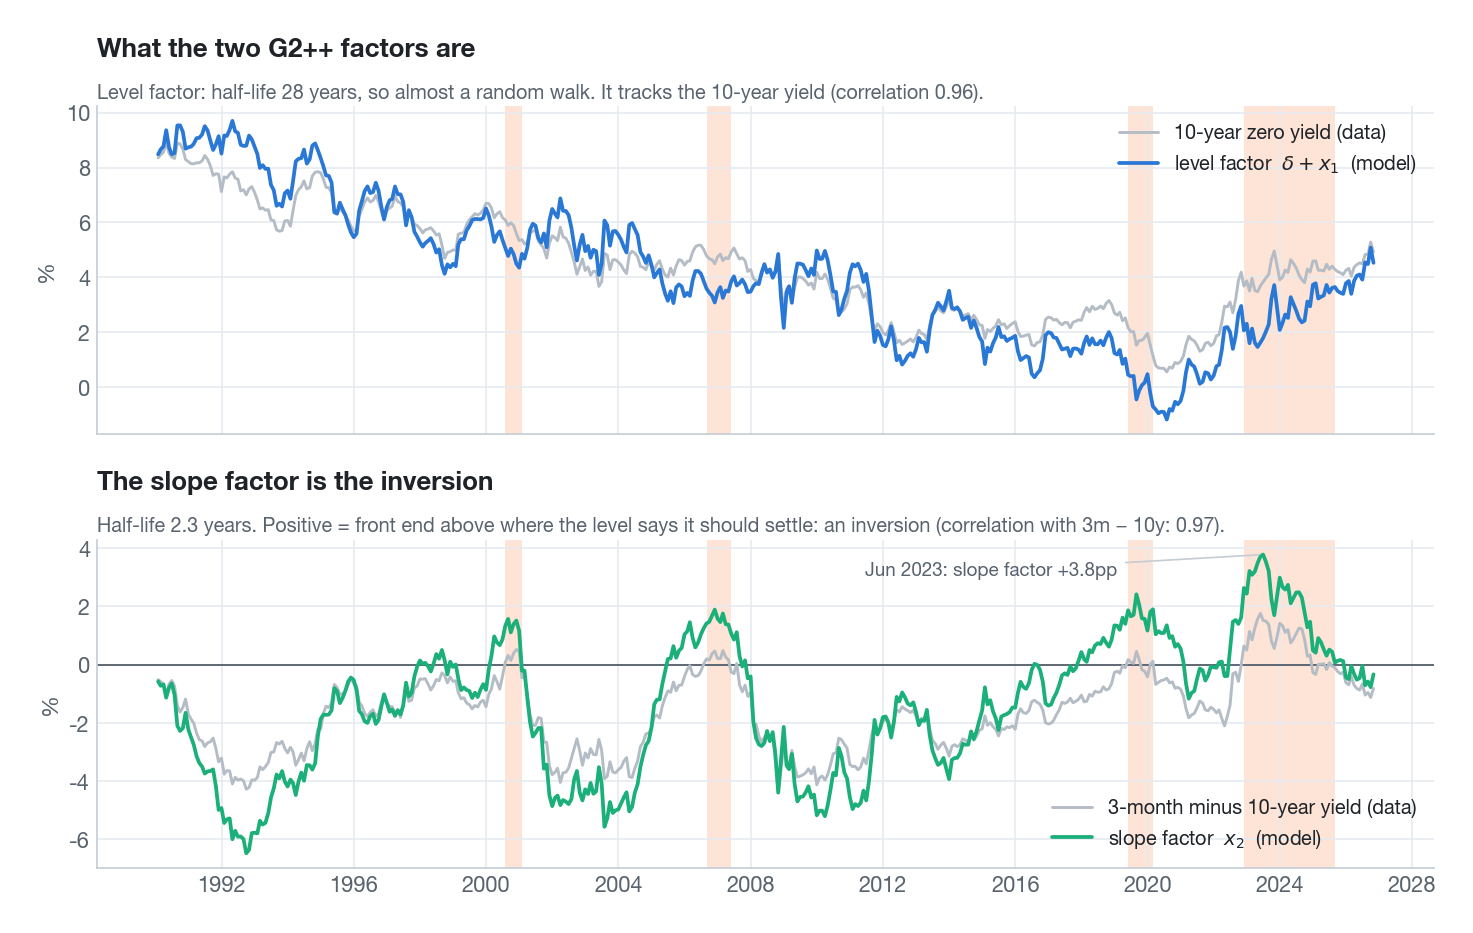
\includegraphics[width=0.60\textwidth]{g2_factors-light.png}
  \caption{The two G2++ factors from the one-parameter-set fit. Top: the level factor tracks the 10-year yield. Bottom: the slope factor tracks the 3-month minus 10-year spread (correlation 0.97) and is positive in every inversion.}
  \label{fig:factors}
\end{figure*}

\begin{figure*}[t]
  \centering
  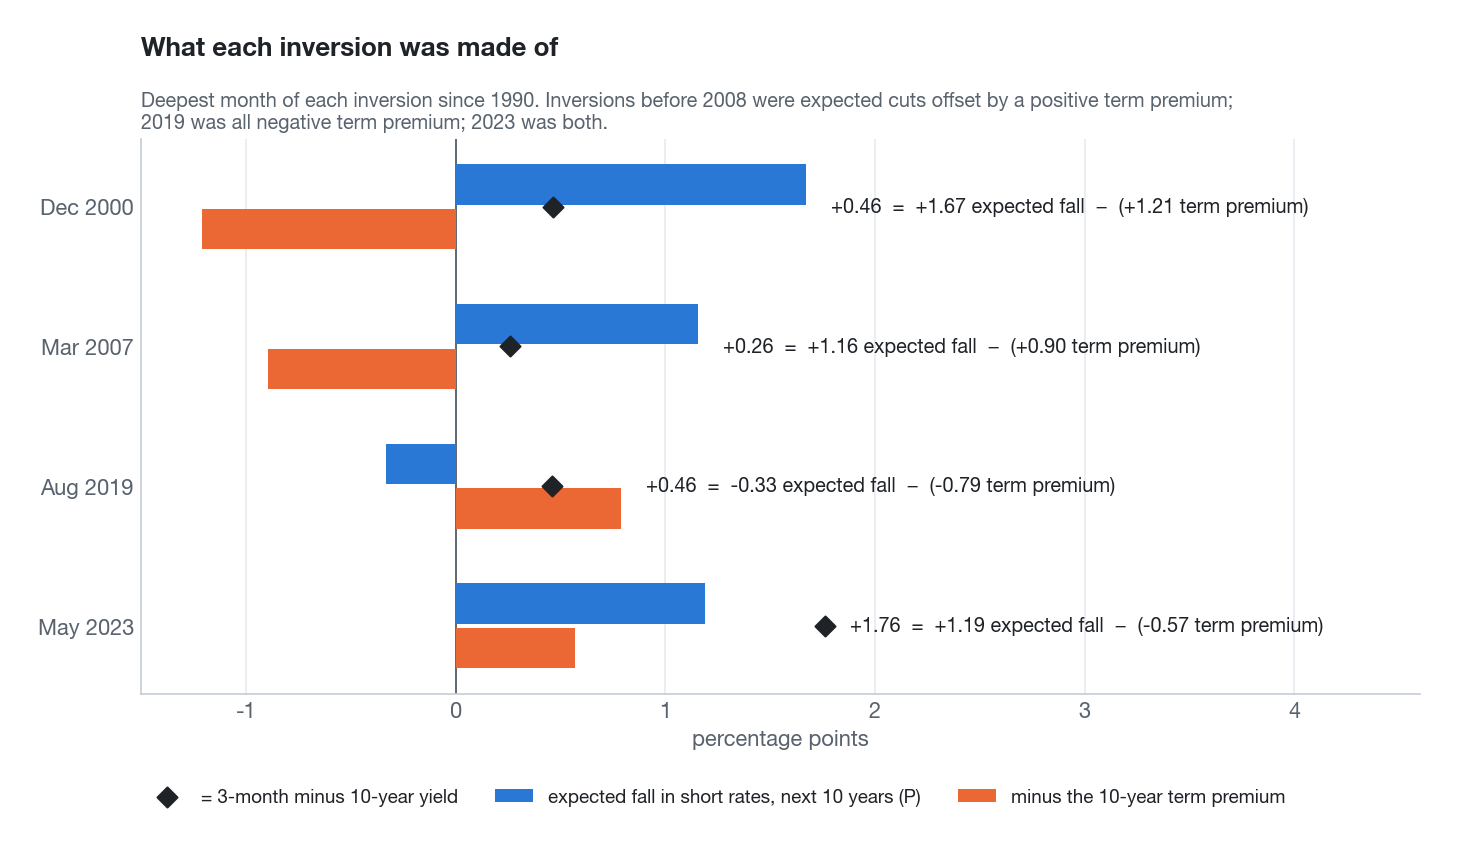
\includegraphics[width=0.56\textwidth]{inversion_decomposition-light.png}
  \caption{At the deepest month of each inversion since 1990, the 3-month minus 10-year spread split into the expected fall in short rates over ten years ($P$) and minus the ten-year term premium.}
  \label{fig:decomp}
\end{figure*}

\paragraph{Real-world dynamics and term premium} Fitted parameters are risk-neutral ($Q$). Following the approach behind the NY Fed's published estimate \citep{acm2013}, we keep the $Q$ loadings and estimate the real-world ($P$) dynamics with a VAR(1) on the monthly factors. The expected average short rate over ten years is the \emph{expectations} part of the ten-year yield; the remainder is the \emph{term premium}.

\paragraph{Announcements} ETF price changes in four liquid funds (SHY, IEI, IEF, TLT, about 2, 5, 8 and 25 years) are converted to yield changes with par-bond durations. We measure yield moves from 8:25 to 8:50 for CPI and jobs reports and from 13:55 to 14:25 for FOMC statements, against the same windows on 281 control days with no announcement.

%==============================================================================
\needspace{12\baselineskip}
\section{Results}

\subsection{Fitting five regimes}

\begin{figure*}[t]
  \centering
  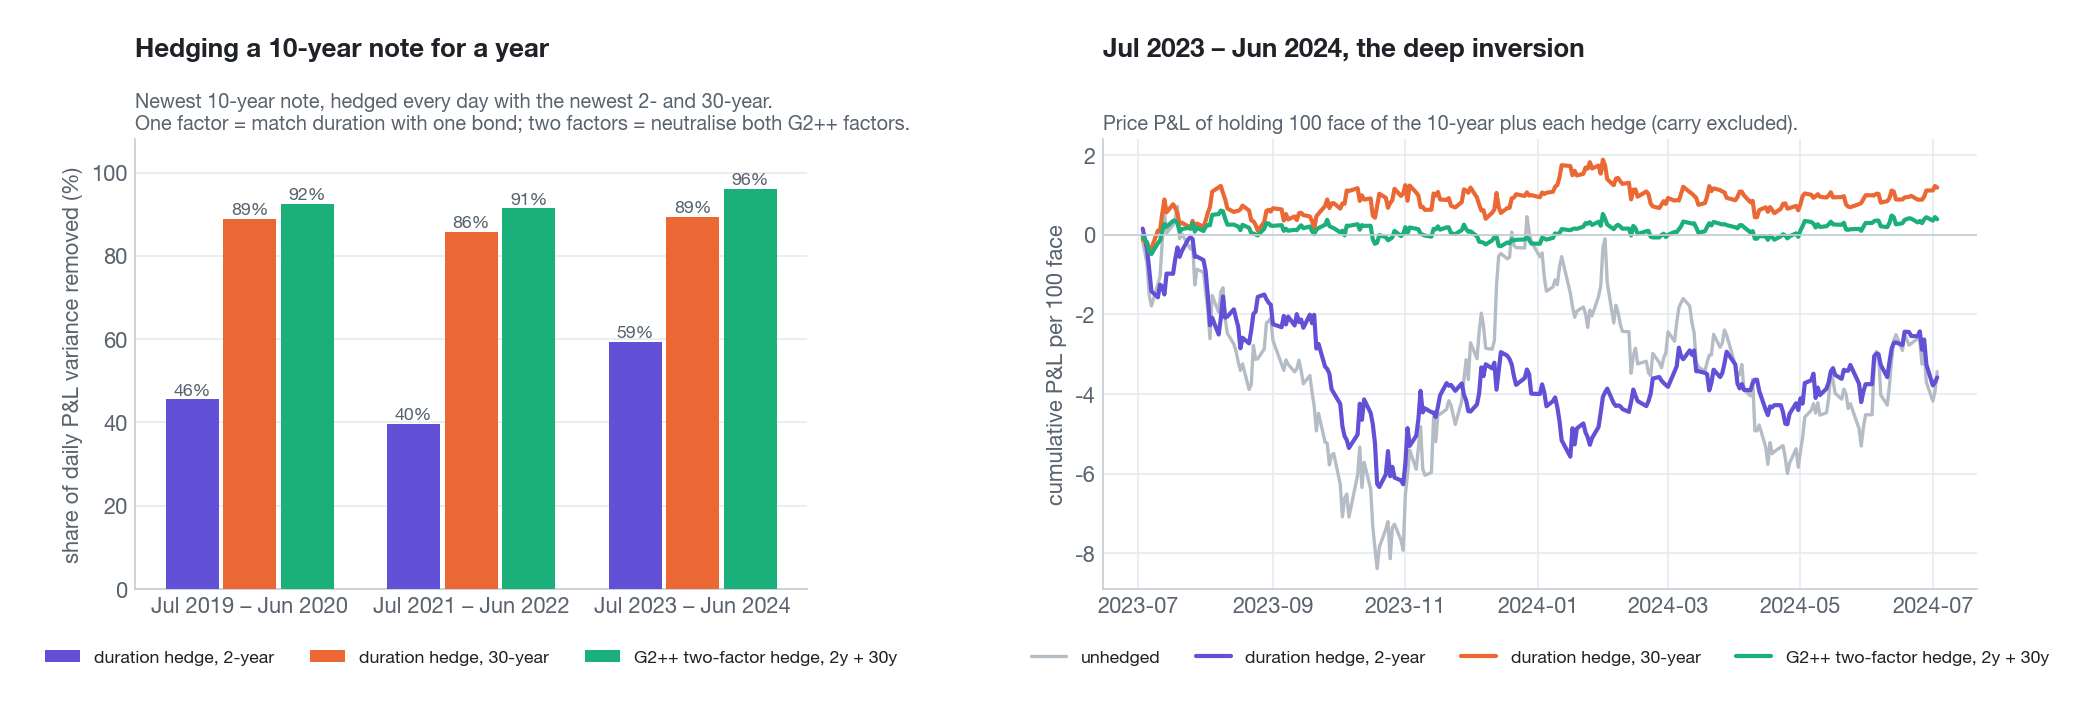
\includegraphics[width=0.80\textwidth]{hedge-light.png}
  \caption{Hedging the newest ten-year note for a year, daily, with the newest 2- and 30-year notes. Left: share of daily P\&L variance removed. Right: cumulative P\&L, Jul 2023--Jun 2024.}
  \label{fig:hedge}
\end{figure*}

\begin{figure*}[t]
  \centering
  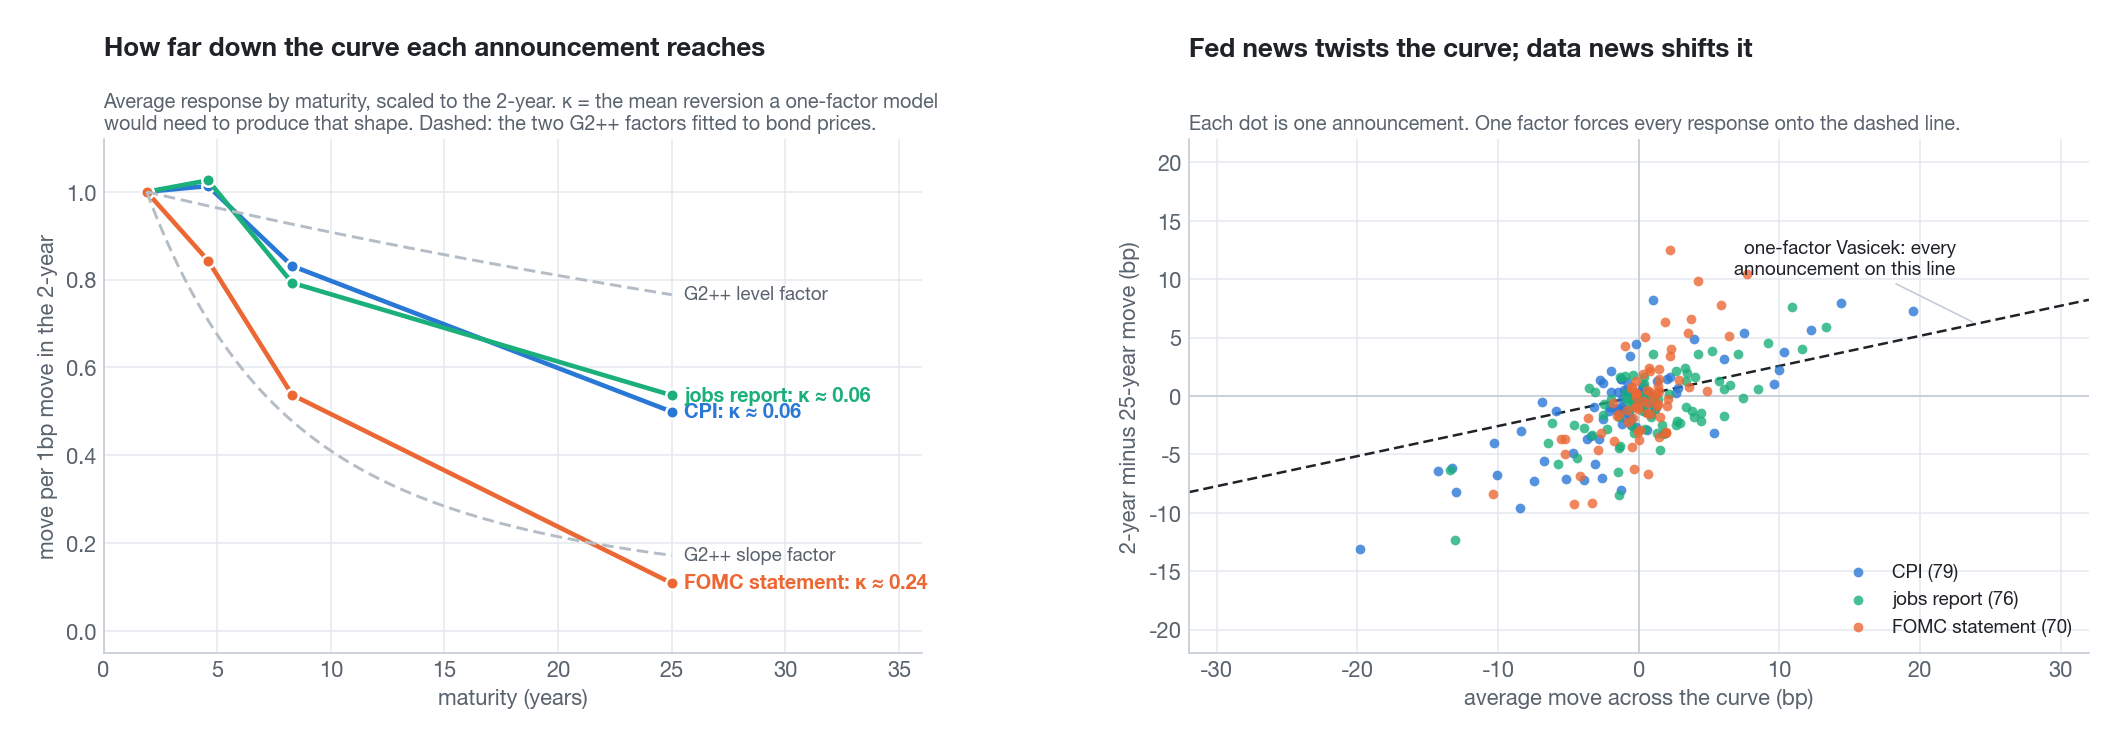
\includegraphics[width=0.80\textwidth]{event_shape-light.png}
  \caption{Left: average response to announcements by maturity, per 1\bp\ at the 2-year, with the two G2++ factor loadings (dashed). Right: each announcement's average move against its 2-year minus 25-year move; one factor would put every point on the dashed line.}
  \label{fig:events}
\end{figure*}

\begin{table}[t]
\centering\small
\setlength{\tabcolsep}{4pt}
\begin{tabular}{@{}lccccc@{}}
\toprule
RMSE (bp) & Dec 06 & Jun 21 & Jun 23 & Sep 24 & Jun 26 \\
\midrule
\multicolumn{6}{@{}l}{\emph{All parameters fitted per date}} \\
Svensson & 2.6 & 2.2 & 6.4 & 4.9 & 3.3 \\
G2++ & 3.5 & 2.2 & 7.9 & 5.1 & 7.0 \\
Vasicek & 8.9 & 5.7 & 14.5 & \textbf{26.4} & 9.4 \\
\midrule
\multicolumn{6}{@{}l}{\emph{One parameter set for all five dates}} \\
G2++ & 5.9 & 8.0 & 13.0 & 18.5 & 10.1 \\
Vasicek & 12.5 & 13.2 & \textbf{50.4} & 31.9 & 35.5 \\
\bottomrule
\end{tabular}
\caption{Yield errors by model and date. CIR is within 1\bp{} of Vasicek on every date.}
\label{tab:rmse}
\end{table}

\begin{takeaway}
Refitted per date, two factors match the best curve-fitter and one factor is 2--5$\times$ worse. With one parameter set for all dates, one factor fails (up to 50\bp) while two factors still fit to 6--18\bp.
\end{takeaway}

\Cref{fig:jun23} and \cref{tab:rmse} summarize the fits. Svensson prices every date to 2--6\bp; its remaining errors come from specific bonds, not from the curve's shape (in June 2023 the old 2036--37 bonds traded about 20\bp\ rich and the 20-year issues about 9\bp\ cheap). Vasicek fails on the U-shaped September 2024 curve, as \eqref{eq:vas} predicts. More tellingly, it fits the inverted dates only with $\sigma$ at its 10\% cap, ten times realistic short-rate volatility, and the steep 2021 curve only with $\theta=18\%$: $\sigma$ and $\kappa$ become shape knobs. In the shared test Vasicek's best compromise is a nearly flat curve on every date. G2++ keeps 6--18\bp, with a near-permanent \emph{level} factor and a \emph{slope} factor that has a 1.7-year half-life.

\needspace{12\baselineskip}
\subsection{One parameter set for 37 years}

\begin{takeaway}
Over 442 months, one factor has a 49\bp\ median error (82\bp\ in inverted months). Two factors have 14\bp, and 12.5\bp\ in inverted months: \emph{no worse} than in normal times.
\end{takeaway}

The monthly fits (\cref{fig:time}) confirm the five-date result. Vasicek is worst exactly when the curve is far from its average shape, in inversions and in very steep periods. G2++ errors rise when rates move fastest (2008--09, 2022), not when the curve inverts. A third, curvature factor (Dynamic Nelson-Siegel) lowers the median to 9\bp. The G2++ factors have clear meanings (\cref{fig:factors}). The level factor (half-life 28 years) tracks the ten-year yield (correlation 0.96). The slope factor (half-life 2.3 years) is positive in every inversion and peaked at $+3.8$ points in 2023, the highest in 37 years. \emph{In this model an inversion is the slope factor far above zero:} the short end sits above where the level says rates will settle, and the model expects it to come down.

\needspace{12\baselineskip}
\subsection{What the inversion priced}

\begin{takeaway}
Half to two-thirds of the May 2023 inversion was expected rate cuts and a third to a half a negative term premium. Earlier inversions were mostly expected cuts (2000, 2007) or mostly term premium (2019).
\end{takeaway}


\begin{table}[h]
\centering\small
\begin{tabular}{@{}lcc@{}}
\toprule
G2++ factors & priced by bonds ($Q$) & history ($P$) \\
\midrule
Level: half-life of a shock & 28 years & 4.4 years \\
Slope: half-life of a shock & 2.3 years & 3.9 years \\
Short-rate volatility & 1.4\% & 0.8\% \\
\bottomrule
\end{tabular}
\caption{Risk-neutral vs.\ real-world factor dynamics. The level gap is the term premium.}
\label{tab:pq}
\end{table}

Bonds price the level factor as nearly permanent, while its history says shocks fade in about 4.4 years (\cref{tab:pq}). That gap is the term premium. Our ten-year premium moves with the NY Fed's ACM estimate (correlation 0.98); it sits 0.9 points higher because our long-run rate is estimated on 1990--2026. \Cref{fig:decomp} splits each inversion. In 2023, 1.2 points came from expected cuts and 0.6 from a negative premium (0.8 and 0.9 on the 1971--2026 sample; 1.1 and 0.7 for the NY Fed), so as a recession signal the inversion was weaker than its depth suggested. Averaged over each episode, past inversions priced cuts of about 0.2 points over the next 12 months and got 1.7--3.6 points, because the cuts were a recession response. In 2022--25 the curve priced 0.5 and got 0.5. From June 2023 the curve priced the 3-month yield at 4.69\% a year later (actual 5.41\%) and 3.86\% three years later (actual 3.83\%): the right destination, a year late.

\needspace{12\baselineskip}
\subsection{Pricing and hedging with the curve}

\begin{takeaway}
The curve prices bonds it was not fitted to almost as well as those it was. Two factors need two hedging bonds, and that hedge removes 91--96\% of a ten-year note's daily risk.
\end{takeaway}

A fitted curve is a discount function: each cash flow is discounted at the zero yield for its date and the values are summed. The same curve and its forward rates price swaps and floating-rate notes: a swap's fixed leg is a coupon bond, and a floating leg is worth par on each reset date. The newest ten-year note on 30 June 2023 (3.375\%, May 2033) is worth 95.70 on the Svensson curve and 95.71 on the shared G2++ curve, against a market price of 96.63. The 11\bp\ gap is the premium investors pay for the newest issues (all four recent ten-year notes were 9--12\bp\ rich), exactly the rich/cheap signal relative-value desks trade. In a five-fold hold-out (fit on 80\% of bonds, price the rest) errors rise by at most 0.2\bp: Svensson 3.9 to 4.0\bp, G2++ 5.1 to 5.3\bp. No model overfits.

\begin{figure*}[t]
  \centering
  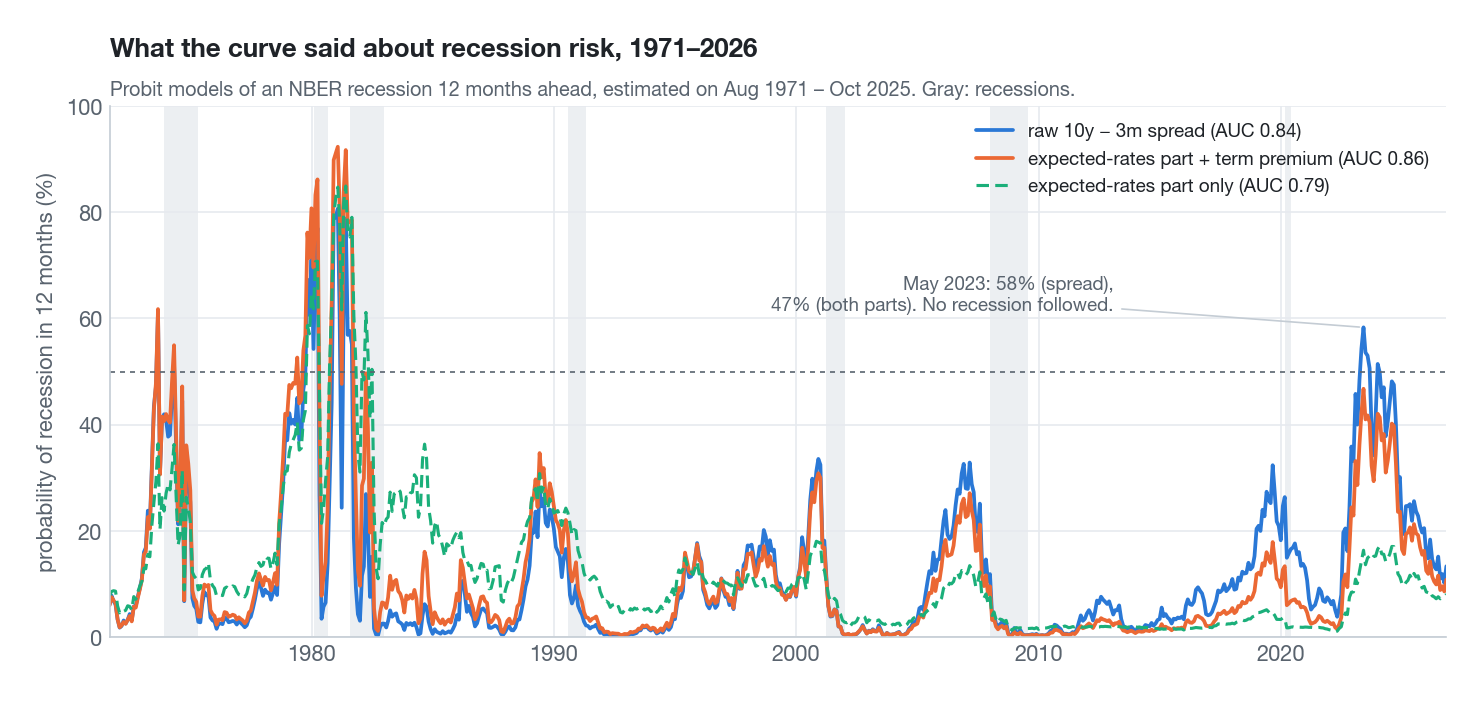
\includegraphics[width=0.70\textwidth]{recession_probability-light.png}
  \caption{Probability of an NBER recession 12 months ahead from probit models estimated on Aug 1971--Oct 2025, using the raw 10-year minus 3-month spread, its expected-rates part, or both parts (expected rates and term premium).}
  \label{fig:recession}
\end{figure*}

\textbf{Hedging} (\cref{fig:hedge}). A bond's G2++ sensitivity to factor $k$ is $-\sum_j CF_j\,P(t_j)\,B_k(t_j)$. Neutralizing both factors with the 2- and 30-year notes removes 91--96\% of the ten-year note's daily P\&L variance over three different years, using actual CRSP prices. A one-bond duration hedge removes 40--59\% with the 2-year and 86--89\% with the 30-year.

\textbf{An option.} G2++ prices a call on a zero-coupon bond in closed form \citep{brigo2006}, and a 100,000-path simulation matches it (at the money: 1.617 $\pm$ 0.008 vs.\ 1.620 per 100). For a one-year call on a ten-year zero, the volatility implied by the curve fit is 62\bp\ a year, about half the 117--125\bp\ the ten-year yield actually moved, so the curve alone would price the option at half. The curve pins down the drift, not the volatility; in practice volatility is calibrated to option prices.

\needspace{12\baselineskip}
\subsection{Robustness: out of sample, back to 1971, and recessions}

\begin{takeaway}
G2++ parameters frozen at 2015 price the 2022--25 inversion out of sample to 11\bp. On 1971--2026 our term premium matches the NY Fed's level. Recession models gave 2023 even odds.
\end{takeaway}

\textbf{Out of sample.} We re-estimated the one-parameter-set models on Aug 1971--Dec 2015 only, froze the parameters, and priced every month from 2016 to 2026. G2++ errors were 13\bp\ (11\bp\ in-sample) and \textbf{11\bp\ in the inverted months of 2022--25}: estimated before the inversion, the model priced it as well as a fit that saw it. Vasicek rose from 54 to 81\bp, and to 119\bp\ in the inversion. Fitted on the two halves of the sample separately, G2++'s mean-reversion speeds are fairly stable but its volatilities and correlation are not, and swapping them costs only 5--7\bp: yields pin down the curve shapes, not the volatilities.

\textbf{Back to 1971.} Re-estimated on 55 years (Aug 1971--Oct 2026), our ten-year term premium matches the NY Fed's in level (1.58 vs.\ 1.58 points on average) as well as in swings (correlation 0.97). The 2023 split moves with it: the negative premium explains 32\% (1990 sample), 52\% (1971 sample) or 39\% (NY Fed) of the inversion.

\textbf{Recessions} (\cref{fig:recession}). A probit of ``recession 12 months ahead'' on the raw spread (7 recessions, AUC 0.84) gives May 2023 a 58\% probability; using its expected-rates part and term premium together fits slightly better (AUC 0.86) and gives 47\%. Both parts are significant, and a low term premium also signals recession. These are the highest readings since the early 1980s, above December 2006 (23--28\%) and August 2019 (18--32\%), which were followed by recessions.

\needspace{12\baselineskip}
\subsection{Bonus: the curve minute by minute}

\begin{takeaway}
Data releases shift the curve (the level factor); Fed statements twist it (the slope factor). The same two factors explain 98--99\% of how the curve jumps within minutes.
\end{takeaway}

In the 25 minutes after the release, the variance of the 2-year yield move is 24 times a normal window for CPI, 14 times for the jobs report and 36 times for FOMC statements. Data news fades along the curve like a factor with mean reversion $\kappa \approx 0.06$, close to the G2++ level factor. Fed news fades like $\kappa \approx 0.24$, close to the slope factor (0.31; \cref{fig:events}). One factor explains 81\% of FOMC responses; the two G2++ factors, never fitted to these data, explain 98\%. Release days add 1--2 days' worth of variance at the front end, about 17\% of the 2-year's annual variance. Adding scheduled jumps on release dates \citep{piazzesi2005} keeps G2++ affine, leaves bond prices unchanged, and makes option volatility step up on each release date.

%==============================================================================
\needspace{12\baselineskip}
\section{Discussion and conclusion}

\paragraph{Answer} A single no-arbitrage model can describe both normal and inverted curves, but not a one-factor one. One factor draws both shapes in theory (inverted when $r>\theta$). In practice it fits only by distorting its volatility and mean reversion date by date, and with fixed parameters it fails, worst in inversions. Two factors, a near-permanent level and a slope that reverts within two to three years, fit 37 years of curves with one parameter set and are as accurate in inversions as in normal times. The same two factors reappear in announcement-day moves and give hedges that remove over 90\% of risk.

\paragraph{Theory vs.\ practice} Three gaps stood out. (i) The volatility that fits a curve's shape is not the volatility of rates: 10\% for Vasicek on inverted dates, and half the realized volatility for the G2++ option. (ii) Bonds price rate shocks as far more persistent than history shows; the difference is the term premium. (iii) The last few basis points are bond-specific (new issues rich, 20-year bonds cheap), and every curve model shares that floor.

\paragraph{The 2022--25 puzzle} Fitted on 1971--2025, recession probits put May 2023 at 47--58\%, the strongest signal since the early 1980s, so the indicator did not break: it called roughly even odds and the less likely outcome occurred. The inversion was deep because the short rate started far above its long-run level after the fastest hiking cycle in 40 years, and because the term premium was negative, not because markets priced a recession. The cuts it priced arrived, a year late. The failed recession signal is less a failure of the curve than a misreading of it.

\paragraph{Limitations and extensions} Our fits only see prices, so volatility should be calibrated to caps or swaptions. The monthly panel is the Fed's smoothed curve rather than individual bonds. The term premium's level depends on the sample's long-run rate, and VARs understate persistence in samples this short. Intraday yields come from ETFs with approximate durations. Natural extensions are the arbitrage-free three-factor model (AFNS) and volatility calibration to option data.

\paragraph{Where it applies} The same fitted model serves four everyday uses. \emph{Relative value:} the gap between a bond's market and model price flags rich and cheap issues (new ten-year notes 9--12\bp\ rich). \emph{Hedging:} two factors call for two hedging bonds, which removed over 90\% of daily risk. \emph{Scenario analysis:} level and slope shocks are natural stress tests, and they match the regulators' parallel and steepener scenarios. \emph{Event risk:} adding jumps on release dates tells an options desk how much more volatility to charge across CPI and FOMC dates.

\begin{keybox}
\textbf{Conclusion.}
\begin{enumerate}
  \item \textbf{One model can describe both normal and inverted curves, if it has two factors.} One factor draws both shapes in theory, but fails with fixed parameters (up to 50\bp; 82\bp\ median in inverted months). Two factors fit 37 years to 14\bp, just as well in inversions.
  \item \textbf{An inversion is the slope factor at an extreme, not a different regime.} In 2023 it was half to two-thirds expected cuts and a third to a half negative term premium. It priced a gradual easing, and recession models gave it about even odds (47--58\%): a coin flip that came up ``no''.
  \item \textbf{The curve prices and hedges bonds well, but not options on its own.} Bonds need only the curve; hedges need one bond per factor; options need volatility calibrated separately.
  \item \textbf{The two factors are real, not a fitting artifact.} Fitted to month-end prices, they also explain 98--99\% of how the curve jumps within minutes of Fed and data news.
\end{enumerate}
\end{keybox}

{\small
\bibliography{refs}
}

%==============================================================================
\needspace{14\baselineskip}
\section*{Use of AI}
{\small\noindent
\begin{tabularx}{\columnwidth}{@{}p{0.27\columnwidth}X@{}}
\toprule
Tool & Claude (Anthropic), through Claude Code \\
\midrule
Used for & Writing the Python scripts that download and clean the data, fit the models and draw the figures; drafting text, which we then edited. \\
Our role & Chose the question, models, dates and tests; checked every result against the data and against published estimates (NY Fed term premium, known market events); reviewed all code and text. \\
Responsibility & All numbers are produced by the project code; any errors are ours. \\
\bottomrule
\end{tabularx}}

\end{document}
